\chapter{Analysis}
\label{chapter:analysis}

\section{Uncertainties}
\label{sec:uncertainties}

A measurement is only useful if we know how well it was made. The following
sections describe the sources of uncertainty in this measurement and estimate
their impact on the final result.

\subsection{Statistical Uncertainties}
\label{ssec:stat_uncertainty}

The statistical uncertainties due to the number of data events are propagated
through the unfolding method using toy MC, as discussed in
\cref{ssec:unfolding_statistical_uncertainties}. For the normalized cross
section measurement, this uncertainty is corrected for the uncertainty on the
total cross section as follows:

\TODO{Understand this formula...}
\begin{equation} \label{eq:stat}
    \left( \errnorm_{i} \right)^{2}
    =
    \left[
    \errabs_{i} \cdot
        \left(
            \frac{1}{\AllBinN} - \frac{\BinN_{i}}{\AllBinN^{2}}
        \right)
    \right]^{2}
    +
    \sum_{i \ne j}
    \left(
        \errabs_{j} \cdot \frac{\BinN_{i}}{\AllBinN^{2}}
    \right)^{2}
\end{equation}

where $\errnorm_{i}$ is the statistical uncertainty for normalized bin $i$,
$\errabs_{j}$ is the statistical uncertainty for bin $j$ in the absolute
distribution, $\BinN_{i}$ is the number of events in bin $i$ in the absolute
distribution, and $\AllBinN$ is the number of events given by the integral of
the absolute distribution. The correction yielded by this formula is small.

The statistical uncertainty ranges from 0.26 to 1.21\% for both the absolute
and normalized cross section measurement. It is one of the dominant
uncertainties for the normalized cross section measurement.

\subsection{Statistical Uncertainties from the Monte Carlo Samples}
\label{ssec:mc_stat_uncertainty}

The \MADGRAPH and \POWHEG signal MC sample have fewer events which pass our
final selection than there are events in the data. These samples are used to
unfold the data and so their statistical uncertainty affects the final
measurement. The affect of the statistical uncertainty on the bin migration
matrix is propagated through to the final result via the use of toy MC as
detailed in \cref{ssec:unfolding_statistical_uncertainties}. The
uncertainty from using this method with the \MADGRAPH sample is 0.1 to 0.2\%
for both the absolute and normalized cross section measurements.

In addition to affecting the unfolding, the low number of events in the MC
affects the efficiency correction discussed in \cref{ssec:eff_correction}
and shown in \cref{fig:average_efficiencies}. These uncertainties vary from
0.3 to 1.3\% for both the absolute and normalized cross section measurements.
These uncertainties are calculated in the same manner for \POWHEG, but the
effect is larger as there are fewer events in that sample.

These two sources of uncertainty are measured separately. The finally
uncertainty due to using a specific signal MC sample is the sum in quadrature
of both of these sources. This combined uncertainty is the dominant uncertainty
for the normalized cross section measurement, having a slightly larger effect
in each \phistar bin than the statistical uncertainty due to the data.

\subsection{Luminosity Uncertainty}
\label{ssec:lumi_uncertainty}

The integrated luminosity is measured at CMS using the occupancy in the pixel
detector during minimum-bias events \cite{cms_lumi_2013}. This luminosity
measurement is calibrated by using van der Meer scans---a method to measure the
beam size in which the two beams are offset and then ``swept'' across each
other as that offset is reduced \cite{vandermeer_1968}.

The integrated luminosity for the run period considered in this analysis is
known to \LumiUncertainty. This uncertainty is taken to be fully correlated
bin-by-bin in \phistar for the absolute cross section measurement, where it is
by far the dominant uncertainty. The luminosity cancels in the normalized
cross section measurement and so the uncertainty only affects the background
subtraction. This effect is negligible compared to the uncertainty already
present due to the background subtraction, which is discussed in
\cref{ssec:background_subtraction_uncertainty}. The large uncertainty on
the luminosity is the primary motivation behind making a normalized cross
section measurement.

\subsection{Pileup Uncertainty}
\label{ssec:pileup_uncertainty}

As discussed in \cref{ssec:monte_carlo}, the high beam intensity at the LHC
leads to multiple proton-proton interactions at each bunch crossing. This is
modeled in MC by overlaying multiple simulated minimum-bias events on top of
each simulated event. The distribution of pileup in MC is reweighted to match
the data distribution based on the calculated instantaneous luminosity and the
inelastic proton-proton cross section. The uncertainty due to this reweighting
process is calculated by varying the inelastic cross section by plus and minus
5\%, recalculating the data distribution of pileup, and reweighting the MC
samples to match this new distribution. The full analysis is then performed
with these MC samples and the differences between the \phistar distributions is
taken as a systematic uncertainty. The pileup uncertainty for the absolute
cross section measurement ranges from 0.21 to 0.58\%, while the uncertainty for
the normalized cross section measurement is between $< 0.01$ and 0.64\%.

\subsection{Trigger, Reconstruction, and Identification Scale Factors Uncertainty}
\label{scale_factor_uncertainty}

Differences between the MC and data are corrected for using scale factors.
Three different sets of scale factors are used to reweight the MC samples:
trigger scale factors (discussed in \cref{ssec:sf_trigger}), reconstruction
scale factors (discussed in \cref{ssec:sf_reconstruction}), and
identification scale factors (discussed in \cref{ssec:sf_id}).

In all three cases, the uncertainties on the scale factors are propagated
through to the final measurement using 500 toy MC variations. In this method,
every toy is constructed by drawing each scale factor from a Gaussian
probability distribution with its mean set to nominal value of the scale factor
and its width set to the quadrature sum of the uncertainties on the scale
factor. Each toy is then used to weight the MC samples used in this analysis,
and the full analysis is performed with that newly weighted samples. The
uncertainty on the final result due to one of the three types of scale factors
is taken to be defined by the central 68.2\% of results from the toys.

This procedure for propagating the uncertainty is performed independently for
each of the three types of scale factors. The total uncertainty due to the
scale factors is the sum in quadrature of the three results. For the absolute
cross section measurement this uncertainty is about 0.4\%, while for the
normalized cross section measurement it ranges from 0.02 to 0.35\%.

\subsection{\texorpdfstring{\pt}{PT} Scale Uncertainty}
\label{ssec:pt_scale_uncertainty}

One of the advantages of the \phistar variable is that it is not computed using
the momentum of the electrons and instead uses only the angles between them,
which are generally better measured. This makes \phistar less sensitive to any
potential problems with the \pt measurement of electrons.

However, the measurement of the \pt of the electrons is used to determine which
events are included in our sample. Therefore, a shift in the \pt scale of the
detector will either add or remove events that have electrons near the \pt
selection requirement boundaries. To determine the uncertainty due to the \pt
scale, we vary the \pt values of all of the electron up and down by 0.3\%,
which is a conservative estimate of the uncertainty on the \pt scale. The
largest difference in each \phistar bin between the nominal result and the
results with the modified \pt scale is taken as the uncertainty in that bin.
The uncertainty due to the \pt scale for the absolute cross section measurement
is 0.07 to 0.17\%, while the uncertainty for the normalized cross section
measure is $< 0.01$ to 0.10\%.

\subsection{Background Subtraction Uncertainty}
\label{ssec:background_subtraction_uncertainty}

The background subtraction, which is discussed in \cref{sec:background},
deals with three separate categories of backgrounds. The uncertainty in
each category is determined with a different method, and these uncertainties
are added in quadrature to determine the total uncertainty due to the
background subtraction.

The first category consists of the various backgrounds with two independent
decay chains each of which can produce a lepton: $\ttbar$, $\W\W$,
$\DYtotautau$, $t\W$, and $\tbar\W$. The contributions from these backgrounds
are estimated by using an \emu control sample as discussed in
\cref{ssec:emu_sample}. The uncertainty from the scale factors derived
using this method are propagated through to the final result using 500 toy MC
variations. For each variation, the scale factors are randomly drawn from a
Gaussian distribution with mean equal to the nominal value of that scale factor
and width equal to the uncertainty on the scale factor. Each toy is then used
to weight the background MC samples  which are then used to perform the
background subtraction. The full analysis is then run with the newly
background-subtracted data samples. The uncertainty due to the subtraction of
this category of background for each bin in \phistar is defined by the spread
of the central 68.2\% values obtained by the toys.

The second category consists of the backgrounds with a real \Z boson: $\Z\Z$
and $\W\Z$. For these samples we can not use the \emu control sample so the
uncertainty is calculated by taking a correlated 20\% uncertainty on the
theoretical cross section and propagating this through to the final result.

The third and final category consists of the \QCDjets and \wjets
backgrounds. The method of estimating this background is discussed in
\cref{ssec:qcd_background}. Instead of taking the uncertainties from the
fit, which would not account for any systematics in the method used, a
conservative 100\% uncertainty is assigned to this category.

The uncertainty due to the background subtraction for the absolute cross
section measurement varies from 0.02 to 0.64\%, and from 0.03 to 0.59\% in the
normalized cross section measurement.

\subsection{PDF and Cross Section Uncertainties}
\label{ssec:pdf_uncertainties}

As discussed in \cref{ssec:parton_model}, the kinematics of the \Z boson
depend on the internal composition and kinematics of the protons as they
collide. The reconstructed \phistar distribution is therefore dependent on the
PDFs used to generate the signal MC sample.

The uncertainty due to this choice of PDF is calculated following the
recommendation of \PDFforLHC working group for the \POWHEG MC signal sample
\cite{botje_2011}. \PDFWeightProducer is used to reweight the \POWHEG sample
using the \CTten PDF set. A total of \num{26} different pairs of weights are
used by the tool to fully account for the uncertainty inherent in the PDF set;
these weights are provided by the \CTten collaboration specifically for this
purpose. Each pair of weights consists of a variation of a PDF parameter, with
one weight corresponding to adjusting the parameter up and the other weight to
down. Each of these weights are used to reweight the \POWHEG sample, and the
analysis is performed with this newly weighted sample. The uncertainty due to
each weight is taken to be the difference with the nominal \phistar
distribution. Two uncertainties are calculated: the one due to all of the
upward parameter adjustments, and one to all the downward parameter
adjustments, where in each case the uncertainties are added in quadrature. The
largest of these two uncertainties for each \phistar bin is taken as the total
uncertainty.

For the \MADGRAPH MC signal sample, which is an LO sample generated with a LO
PDF, the uncertainties can not be calculated in this manner. Instead, the PDF
includes an uncertainty on the cross section which is used to scale the sample
as calculated by \FEWZ. This uncertainty is propagated through the analysis be
reweighting the \MADGRAPH with this uncertainty both added and subtracted from
the theoretical cross section. The difference in the final \phistar
distribution is taken as the uncertainty due to the \FEWZ cross section. This
uncertainty is the dominant uncertainty from the \MADGRAPH sample.

\subsection{Final State Radiation Uncertainties}
\label{ssec:fsr_uncertainties}

FSR, where an electron radiates a photon, is discussed in
\cref{sec:electron_dressing}. These photons can affect the reconstruction
of the \Z, but this is taken into account during the unfolding as discussed in
\cref{sec:unfolding}. Hence, uncertainties in the modeling of FSR affect
the unfolding and the final measurement.

The uncertainty is calculated using the \FSRWeightProducer, which augments the
\PYTHIA QED calculation with exact $\BigO{\alpha}$ and $\alpha(\pt^{2})$
couplings and reweights the MC sample as if it had been produced with these
calculations from the start. The effect of this reweighting on the final
\phistar distribution is $\le 0.34\%$ for the absolute cross section
measurement and $\le 0.03\%$ for the normalized cross section measurement.

%\subsection{Electron Angular Position Uncertainty}
%
%Since \phistar depends on the angles between the two electrons, it is sensitive
%to mismeasurement of these angles. As discussed in
%\cref{sec:electron_reconstruction}, the position of a reconstructed
%electron comes from the tracker, and therefore misalignment of the tracker
%would lead to a systematic uncertainty on the angle measurement. The magnitude
%of this systematic is estimated by using the position of the ECAL supercluster
%associated with the electron to calculate the electron's position instead of
%using the track. The new supercluster-only position is then used to calculate a
%new \phistarSC that does not depend on the alignment of the tracker.
%
%The position of the supercluster does not take into account the amount the
%bending of the electron due to the magnetic field. While $\eta$ is unchanged by
%the pretense of the field, $\phi$ is changed. A correction is applied to $\phi$
%to find the angle at the interaction point, $\phizero$, based on the angle of
%the supercluster, $\phisc$. This correction is given by
%\cref{eq:b_field_correction} where $q$ is the charge of the electron, \pt is
%the transverse momentum of the electron, $B$ is the magnitude of the magnetic
%field, and \Reffective is the effective radius of ECAL as a function of $\eta$
%and $\theta$ as given in \cref{eq:effective_radius}. The charge and momentum
%come from the electron matched to the supercluster, and although they are
%determined in combination with the tracker, they are far less susceptible to
%the small scale misalignments of the tracker that we are considering.
%
%\begin{equation}\label{eq:b_field_correction}
%    \sin \left( \phisc - \phizero \right)
%    =
%    - \Reffective \frac{q B}{2 \pt}
%\end{equation}
%
%\begin{equation}\label{eq:effective_radius}
%    \Reffective
%    =
%    \left\{
%        \begin{array}{ll}
%            1.29 \meters & \text{if } |\eta| < 1.4442 \\
%            3.14 \meters \times \tan \left(\coord{\theta}\right) & \text{otherwise}
%        \end{array}
%    \right.
%\end{equation}
%
%The resulting \phistarSC distribution is compatible within statistical
%uncertainties with the \phistar distribution and so no systematic uncertainty
%is assigned for the angular position.

\subsection{Uncertainty from Four Vector Corrections}
\label{four_vector_uncertainty}

The \mee distribution in the \MADGRAPH signal MC sample does not precisely
match the distribution in data, as seen in \cref{fig:z_mass}. This
discrepancy remains even after applying the various energy and momentum
corrections to the electrons discussed in \cref{sec:corrections}. In order
to determine the effect this has on the final measurement, the \MADGRAPH signal
MC sample is reweighted to remove this difference. The ratio between the
nominal \phistar value and the value derived after this reweighting is shown in
\cref{fig:z_mass_reweighted}. The circular points show the ratio of the
reconstructed \phistar distributions, while the square points show the ratio of
the generated \phistar distributions. The errors are binomial. Most of the
points are consistent with \num{1}, and so no systematic uncertainty is
assigned for this disagreement.

\begin{figure}[!htbp]
    \centering
    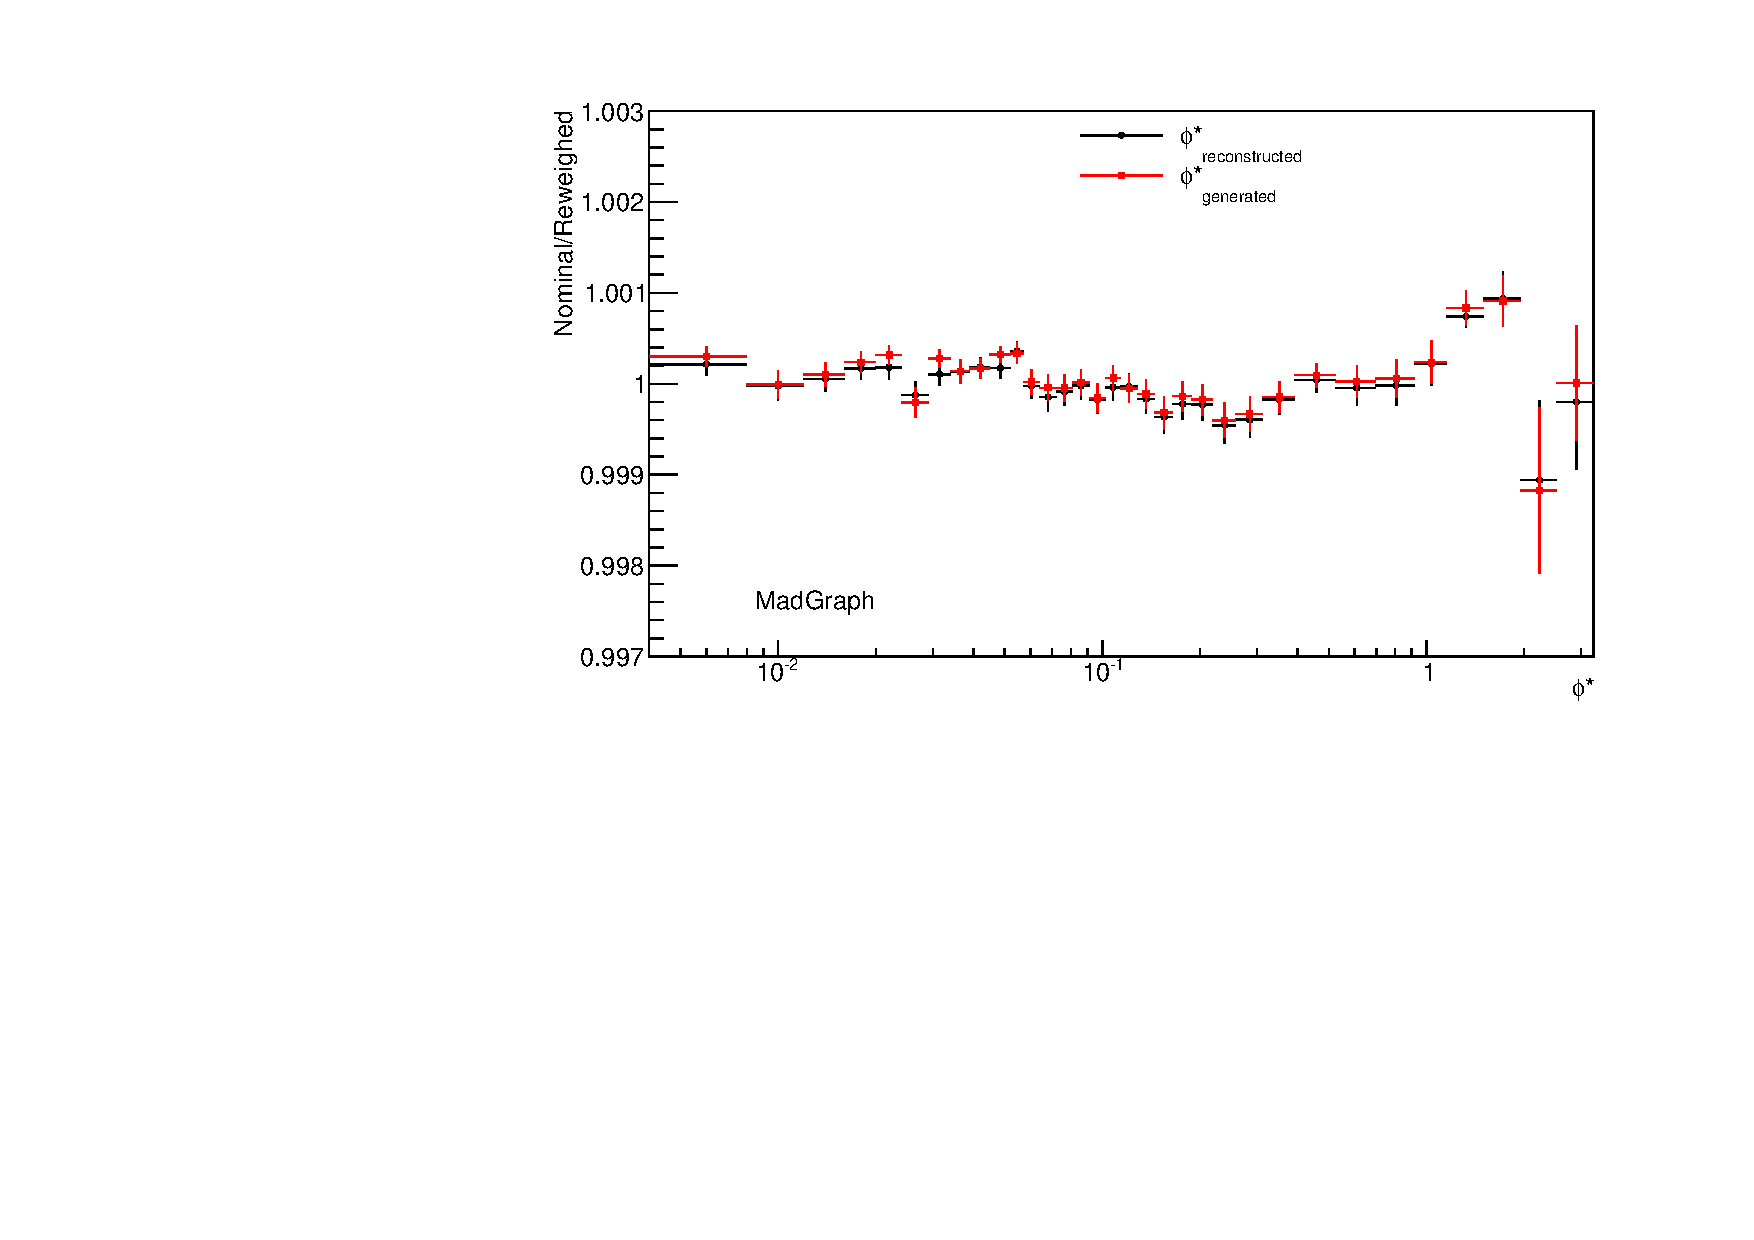
\includegraphics[width=\textwidth]{figures/ZMass_reweighed.pdf}
    \caption[
        The ratio of \phistar in \MADGRAPH before and after reweighting to
        remove the differnce in the \mee distribution between MC and data.
    ]{
        The ratio of \phistar in \MADGRAPH before and after reweighting to
        remove the difference in the \mee distribution between MC and data seen
        in \cref{fig:z_mass}. The circular points are the ratio in the
        reconstructed quantity, while the square points are the ratio in the
        generated quantity. The uncertainties are binomial.
    }
    \label{fig:z_mass_reweighted}
\end{figure}

Likewise, the \Z \rapidity distribution in \MADGRAPH does not match the
distribution in data, as seen in \cref{fig:z_rapidity}. The same
reweighting procedure as is performed for the \mee case above is used here to
force the distributions to agree. The ratio between the nominal \phistar value
and the value derived after this reweighting is shown in
\cref{fig:z_rapidity_reweighted}.
The circular points show the ratio of the
reconstructed \phistar distributions, while the square points show the ratio of
the generated \phistar distributions. The disagreement is on the order of
0.05\% for most of the distribution, increasing to 0.4--0.5\% in the highest
\phistar bins. Although this is larger than the effect seen in the \mee
reweighting, it is much smaller than the statistical uncertainties and so is
not included in the final results.

\begin{figure}[!htbp]
    \centering
    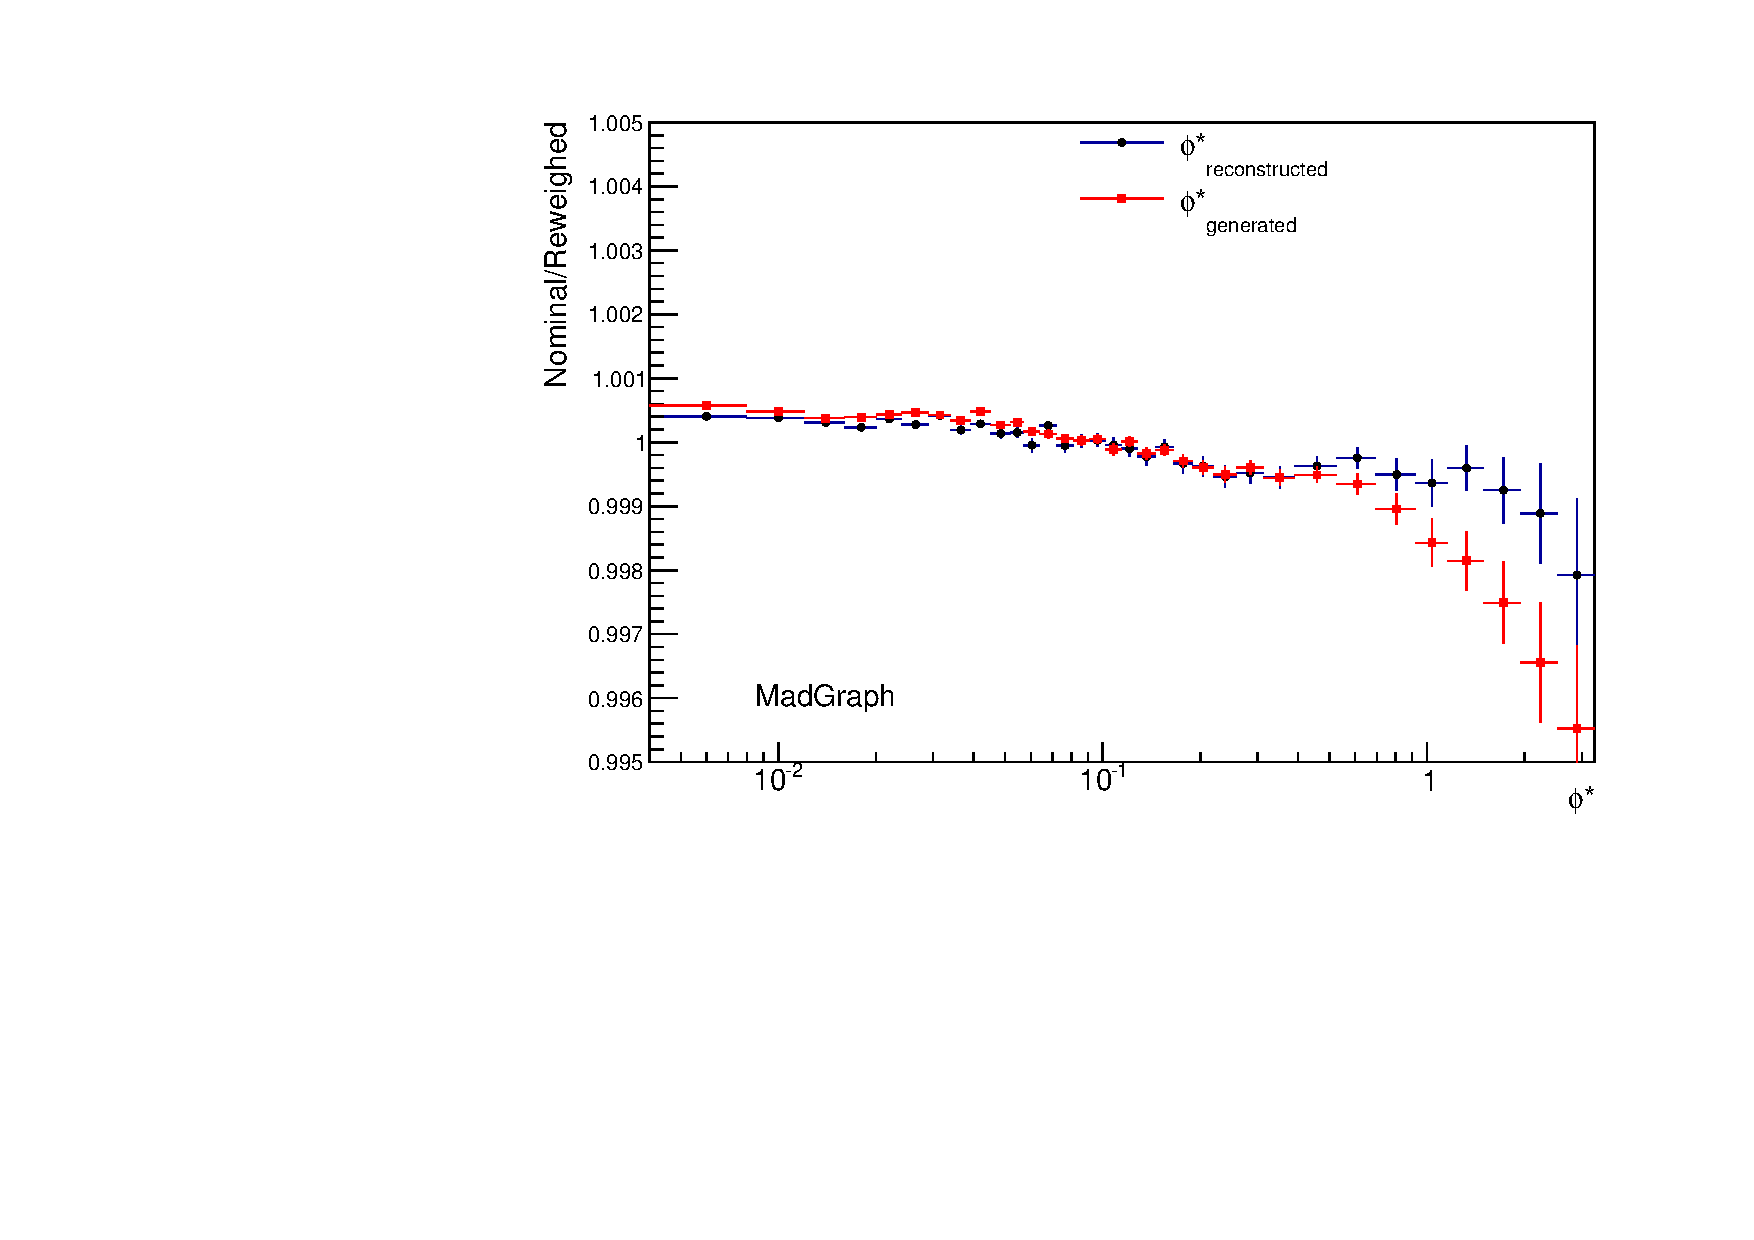
\includegraphics[width=\textwidth]{figures/ZY_reweighed.pdf}
    \caption[
        The ratio of \phistar in \MADGRAPH before and after reweighting to
        remove the differnce in the \rapidity distribution between MC and data.
    ]{
        The ratio of \phistar in \MADGRAPH before and after reweighting to
        remove the difference in the \rapidity distribution between MC and data
        seen in \cref{fig:z_rapidity}. The circular points are the ratio in
        the reconstructed quantity, while the square points are the ratio in
        the generated quantity. The uncertainties are binomial.
    }
    \label{fig:z_rapidity_reweighted}
\end{figure}

\section{Uncertainty Figures}

The values of the various uncertainties in each \phistar bin are presented in
the figures that follow. \Cref{fig:sys_uncert_norm} shows the uncertainties in
the normalized \phistar cross section in data unfolded with \MADGRAPH while
\cref{fig:sys_uncert_norm_powheg} shows the uncertainties in the data unfolded
with \POWHEG. The uncertainties on the normalized \phistar cross section in
\MADGRAPH and \POWHEG are shown in
\cref{fig:madgraph_uncert_norm,fig:powheg_uncert_norm}, respectively. All of
these values are presented in tables in \cref{app:uncertainty_tables}. Figures
showing the uncertainties for the absolute \phistar cross sections are
presented in \cref{app:dressed_measurements}.

% Normalized

% fig:sys_uncert_norm
\begin{figure}[!p]
    \centering
    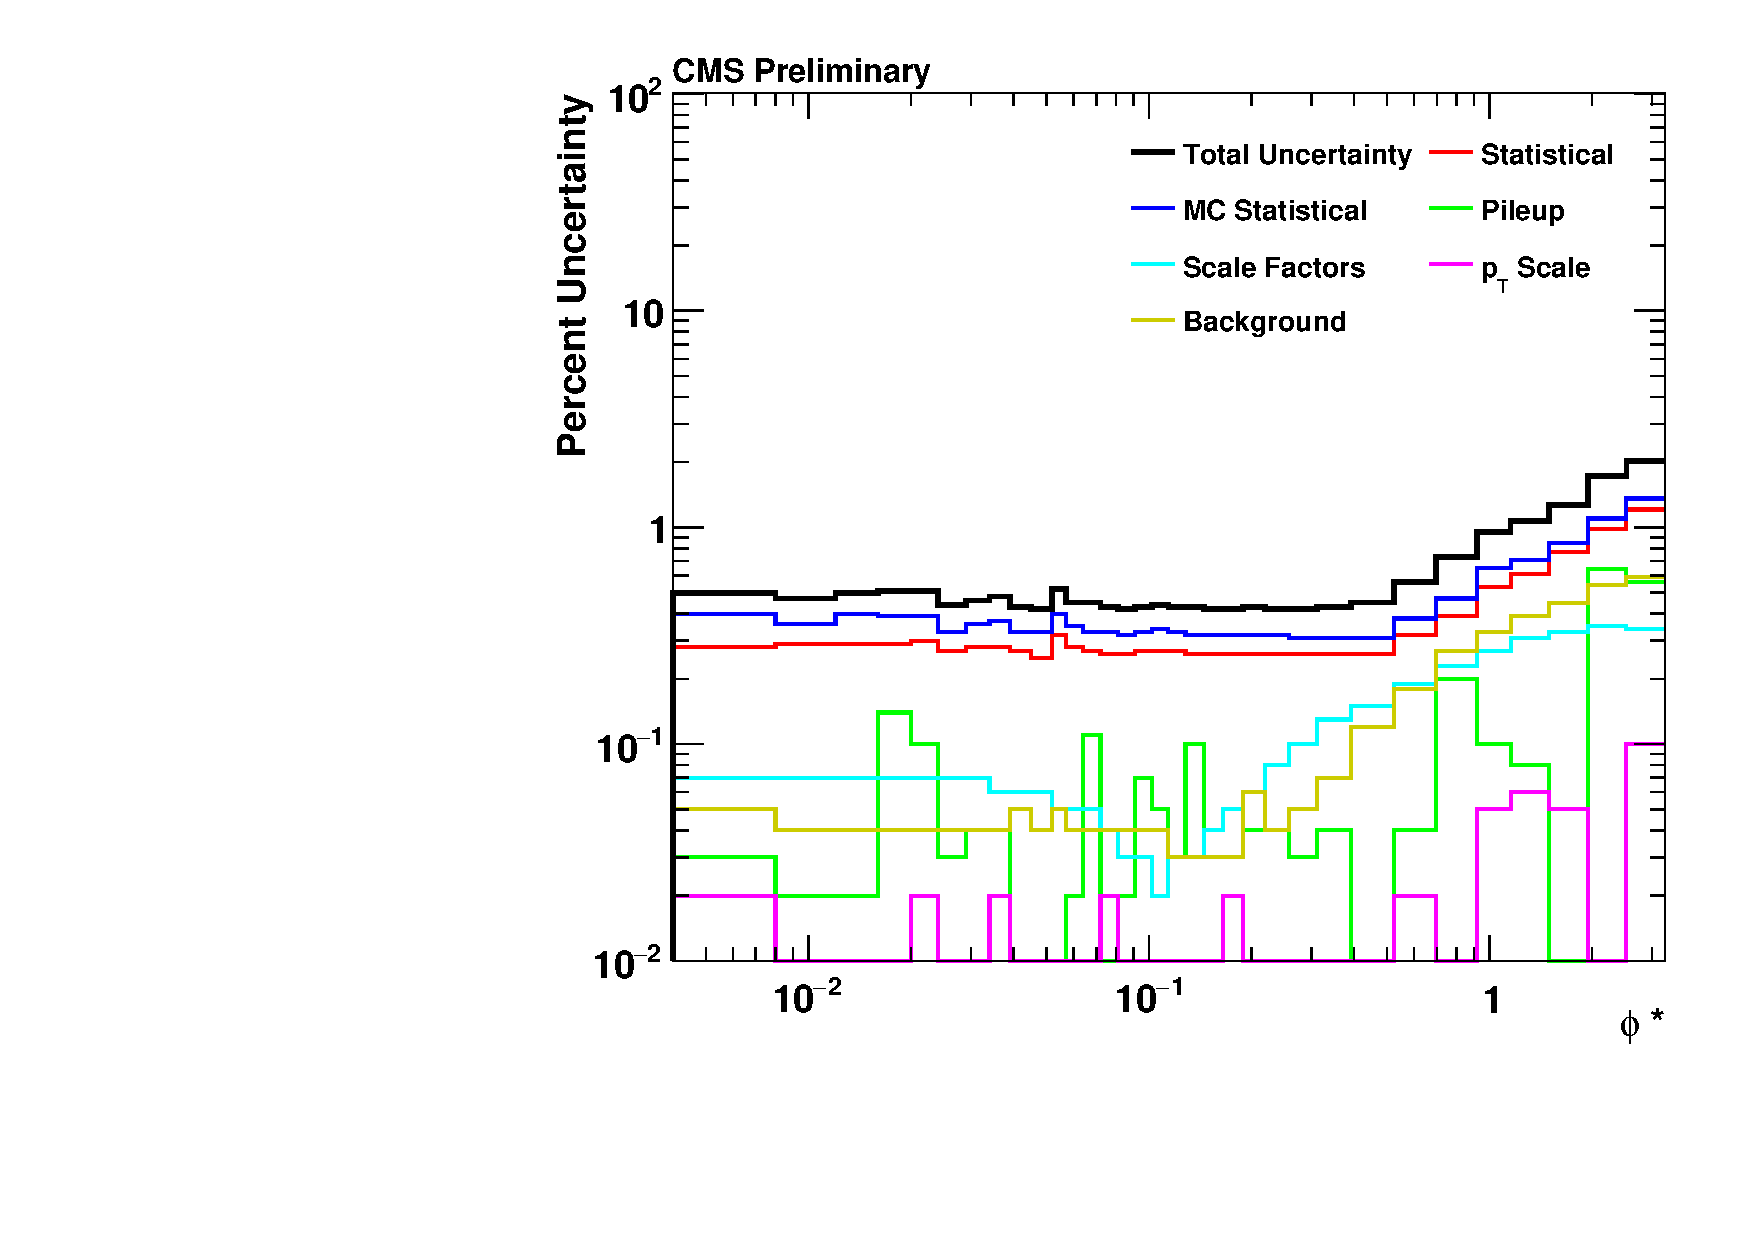
\includegraphics[width=\textwidth]{figures/data_uncertainty_normalized.pdf}
    \caption[
        Fractional errors for the normalized cross section measurement
        made with data unfolded with \MADGRAPH.
    ]{
        Fractional errors (in \%) for the normalized cross section measurement
        made with data unfolded with \MADGRAPH. The total value is the sum in
        quadrature of all the other values. These uncertainties are also
        presented in tabular form in \cref{tab:sys_uncert_norm}.
    }
    \label{fig:sys_uncert_norm}
\end{figure}


% fig:sys_uncert_norm_powheg
\begin{figure}[!p]
    \centering
    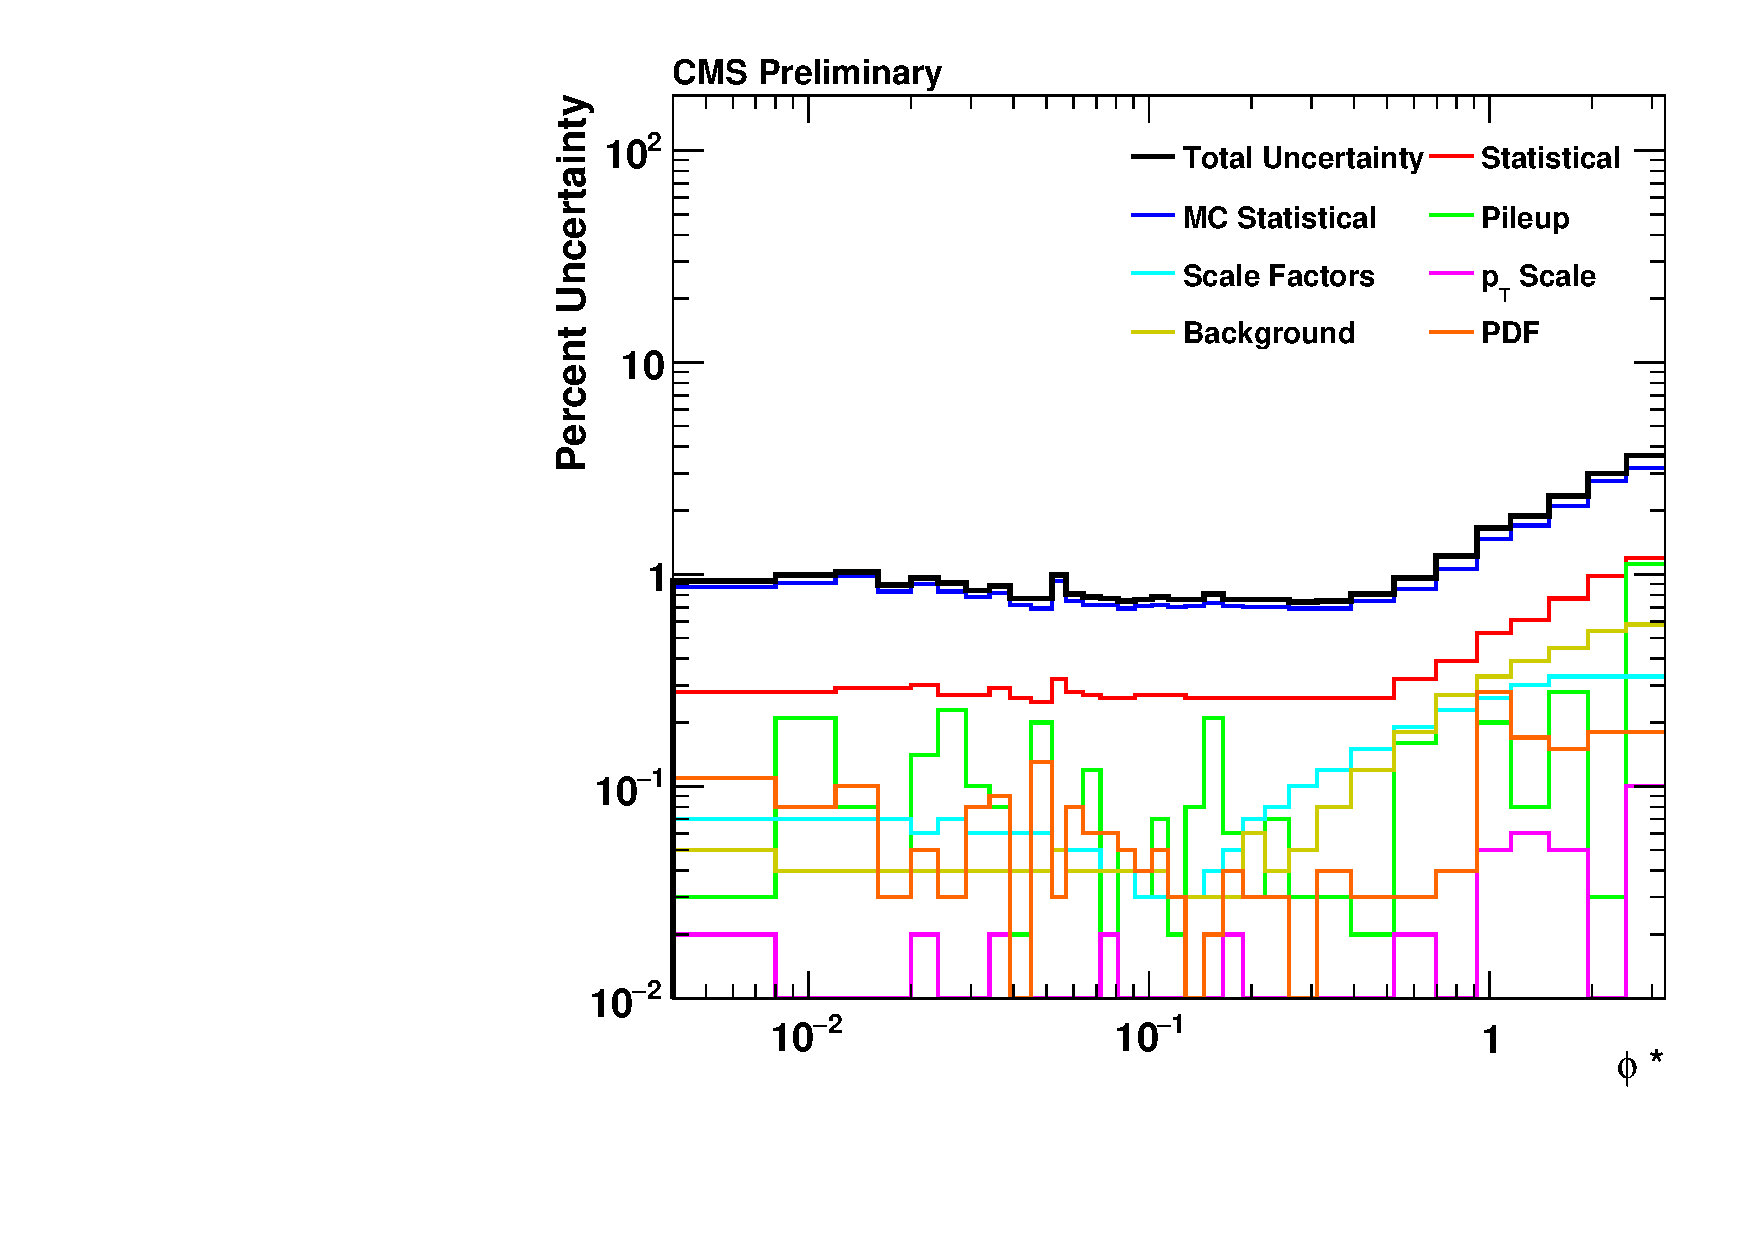
\includegraphics[width=\textwidth]{figures/data_uncertainty_normalized_powheg_unfolded.pdf}
    \caption[
        Fractional errors for the normalized cross section measurement
        made with data unfolded with \POWHEG.
    ]{
        Fractional errors (in \%) for the normalized cross section measurement
        made with data unfolded with \POWHEG. The total value is the sum in
        quadrature of all the other values. These uncertainties are also
        presented in tabular form in \cref{tab:sys_uncert_norm_powheg}.
    }
    \label{fig:sys_uncert_norm_powheg}
\end{figure}


% fig:madgraph_uncert_norm
\begin{figure}[!p]
    \centering
    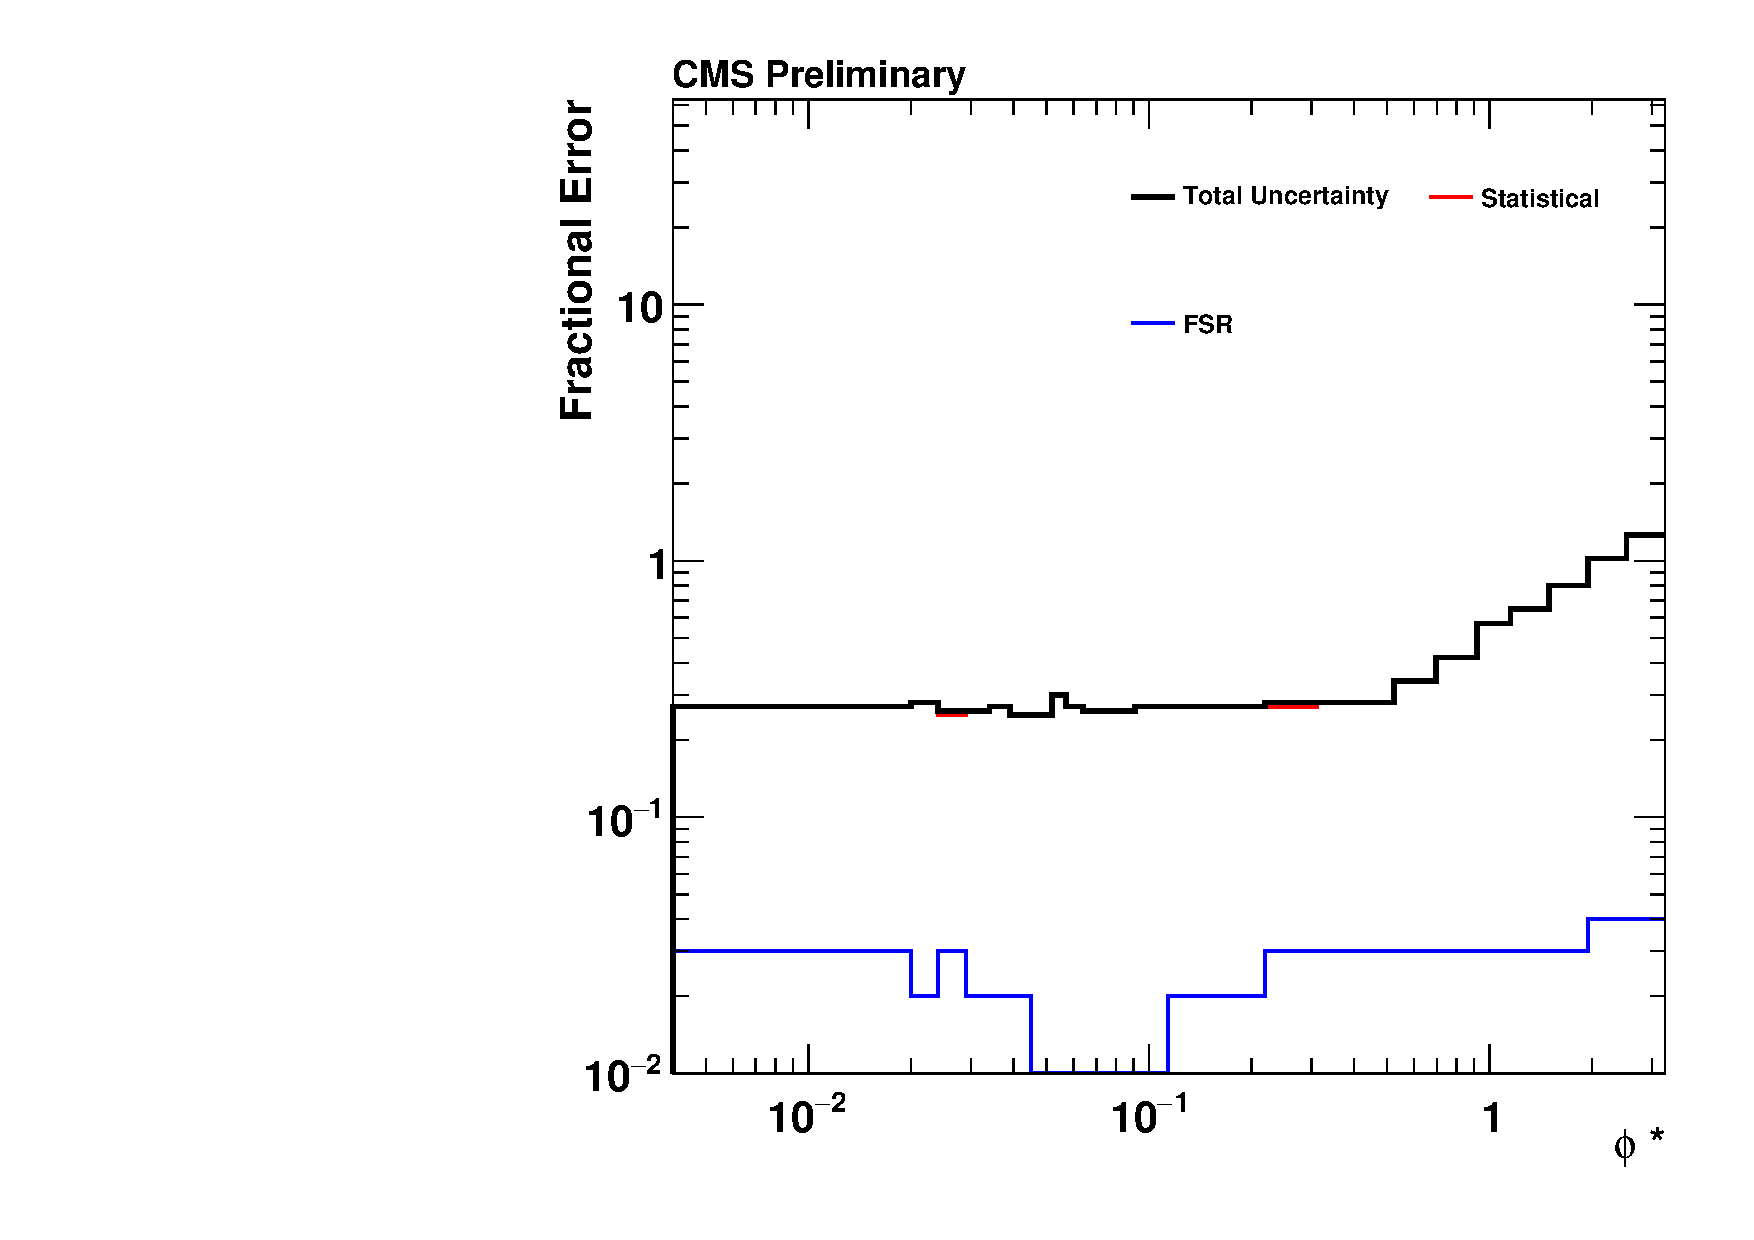
\includegraphics[width=\textwidth]{figures/madgraph_uncertainty_normalized.pdf}
    \caption[
        The uncertainties for the normalized cross section from the \MADGRAPH
        MC sample.
    ]{
        The uncertainties (in \%) for the normalized cross section from the
        \MADGRAPH MC sample. These uncertainties are also presented in tabular
        form in \cref{tab:madgraph_uncert_norm}.
    }
    \label{fig:madgraph_uncert_norm}
\end{figure}


% fig:powheg_uncert_norm
\begin{figure}[!p]
    \centering
    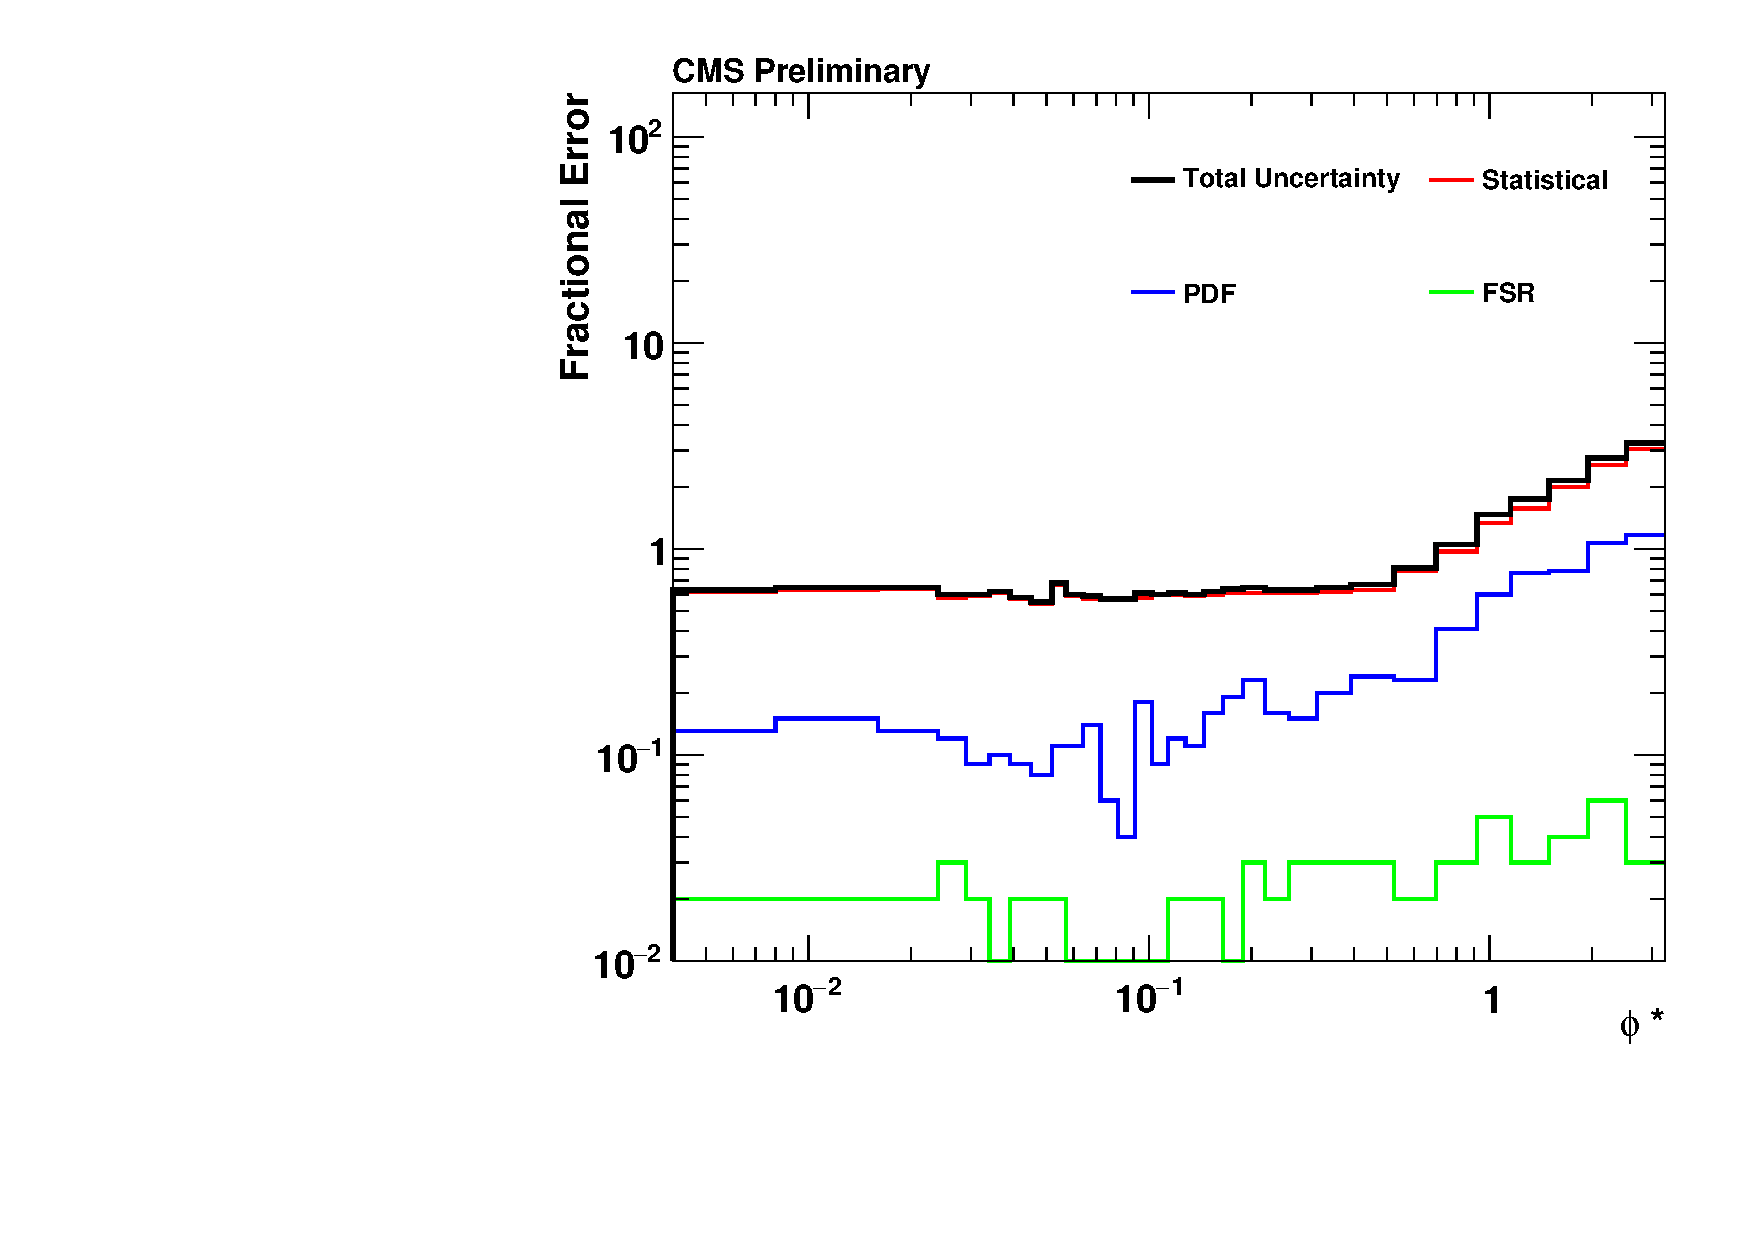
\includegraphics[width=\textwidth]{figures/powheg_uncertainty_normalized.pdf}
    \caption[
        Fractional errors for the normalized cross section from the
        \POWHEG MC sample.
    ]{
        Fractional errors (in \%) for the normalized cross section from the
        \POWHEG MC sample. These uncertainties are also presented in tabular
        form in \cref{tab:powheg_uncert_norm}.
    }
    \label{fig:powheg_uncert_norm}
\end{figure}


\section{Results}
\label{sec:results}

Presented below are our normalized cross section measurements of the
differential \phistar cross section for \Z bosons decaying to an electron pair
in the detector region defined in \cref{sec:acceptance}. Absolute cross
sections are presented in \cref{app:dressed_measurements}. Two sets of data
are used to make the measurement, one unfolded with \MADGRAPH and one unfolded
with \POWHEG; these sets are otherwise identical. The data distributions of
\phistar are compared to the distributions from both the \MADGRAPH MC signal
sample and the \POWHEG MC signal sample.

\subsection{Normalized Differential Cross Section}
\label{ssec:results_norm}

The normalized differential cross section measurement using data unfolded with
\MADGRAPH is shown in \cref{fig:results_norm} and given in tabular form in
\cref{tab:results_norm}. The lower plot in \cref{fig:results_norm} is
shown in more detail in \cref{fig:results_ratio_norm}. As the luminosity
has canceled out in the normalization, the primary uncertainty on the data is
now the statistical uncertainty from the \MADGRAPH sample used to unfold it.
The limit number of events in the MC samples is also the primary uncertainty on
the \MADGRAPH distribution and the \POWHEG distribution.

% fig:results_norm and fig:results_ratio_norm
\begin{figure}[!p]
    \centering
    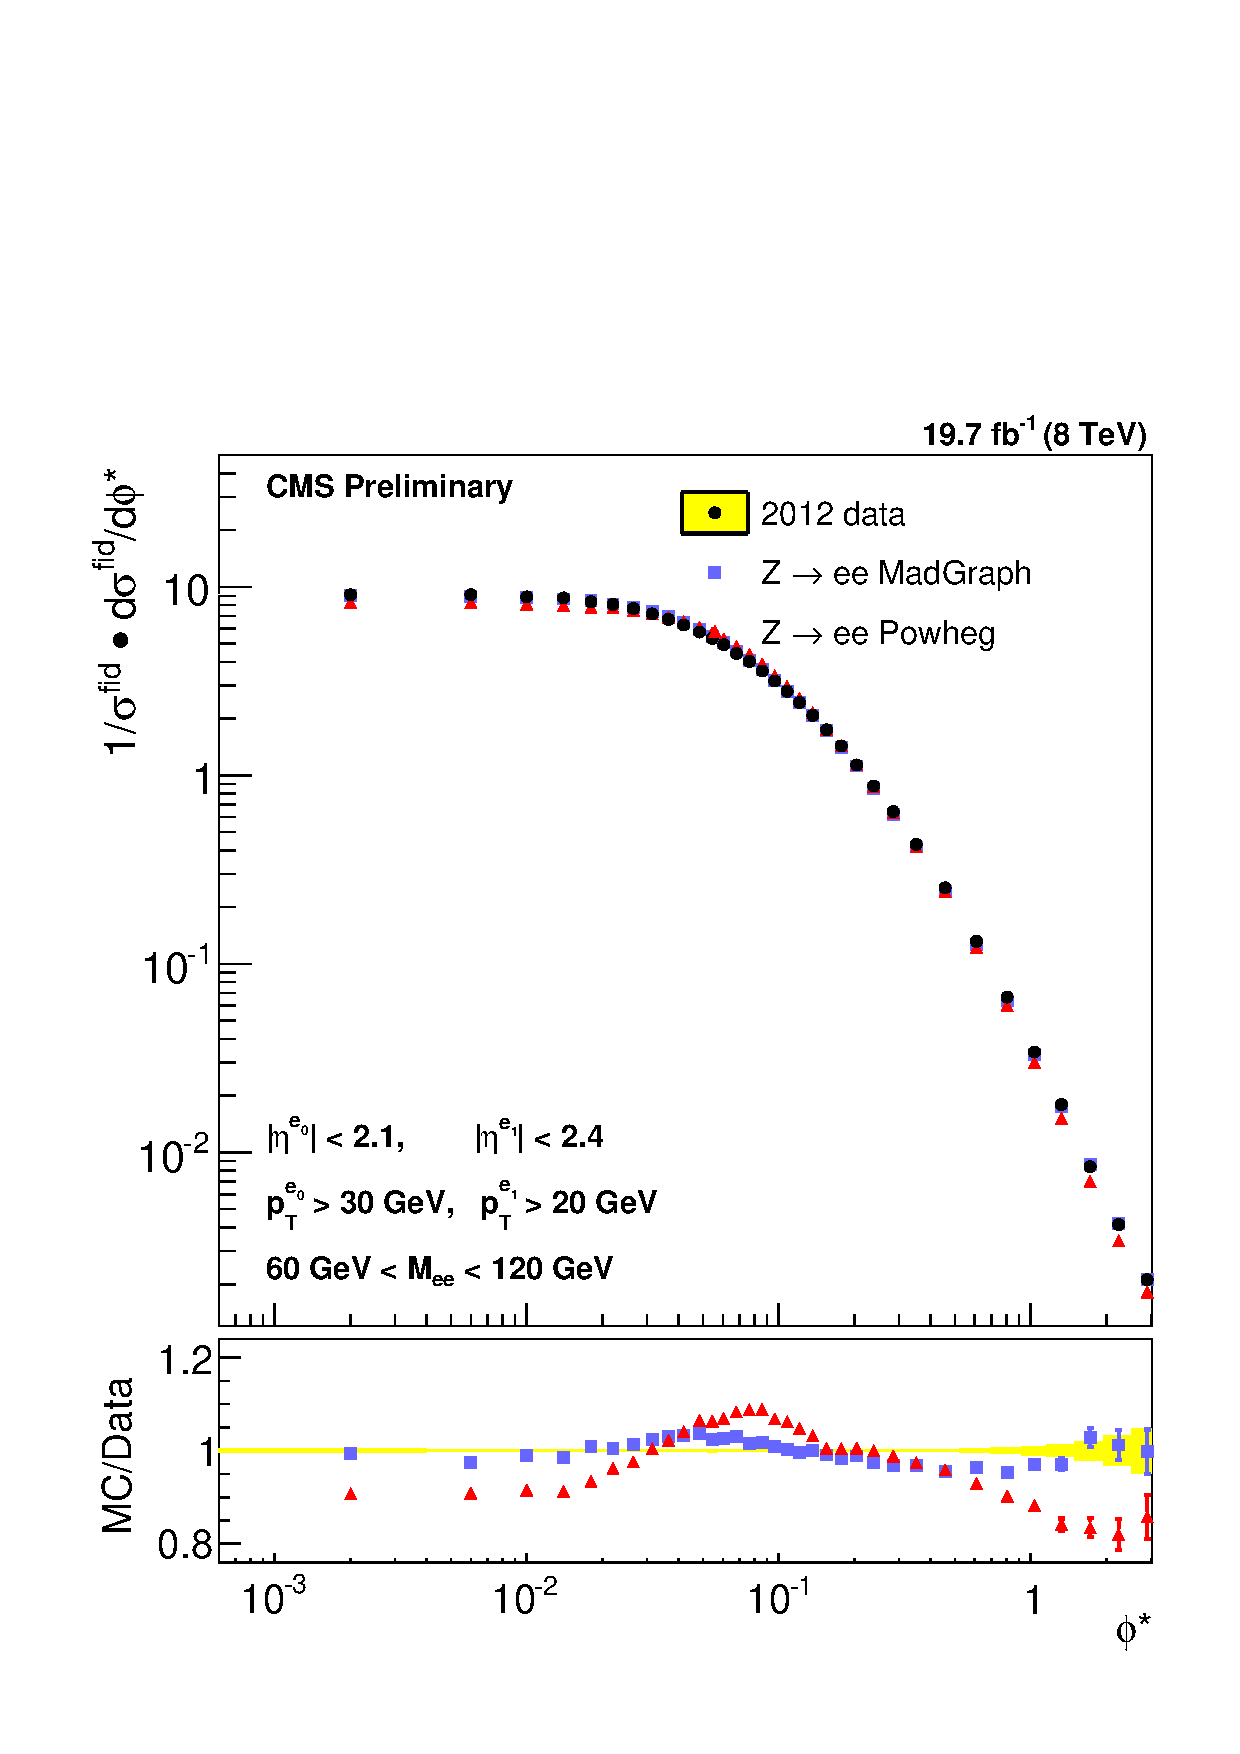
\includegraphics[width=\textwidth]{figures/ZShape_elec_Norm_Dressed.pdf}
    \caption[
        The absolute differential cross section with respects to \phistar for
        \Ztoee events in our fiducial region from data unfolded with \MADGRAPH,
        and the same distributions in \MADGRAPH and \POWHEG.
    ]{
        The absolute differential cross section with respects to \phistar for
        \Ztoee events in our fiducial region from data unfolded with \MADGRAPH,
        and the same distributions in \MADGRAPH and \POWHEG. A close up of the
        lower plot is shown in \FIG~\ref{fig:results_ratio_norm}.
    }
    \label{fig:results_norm}
\end{figure}

\begin{figure}[!p]
    \centering
    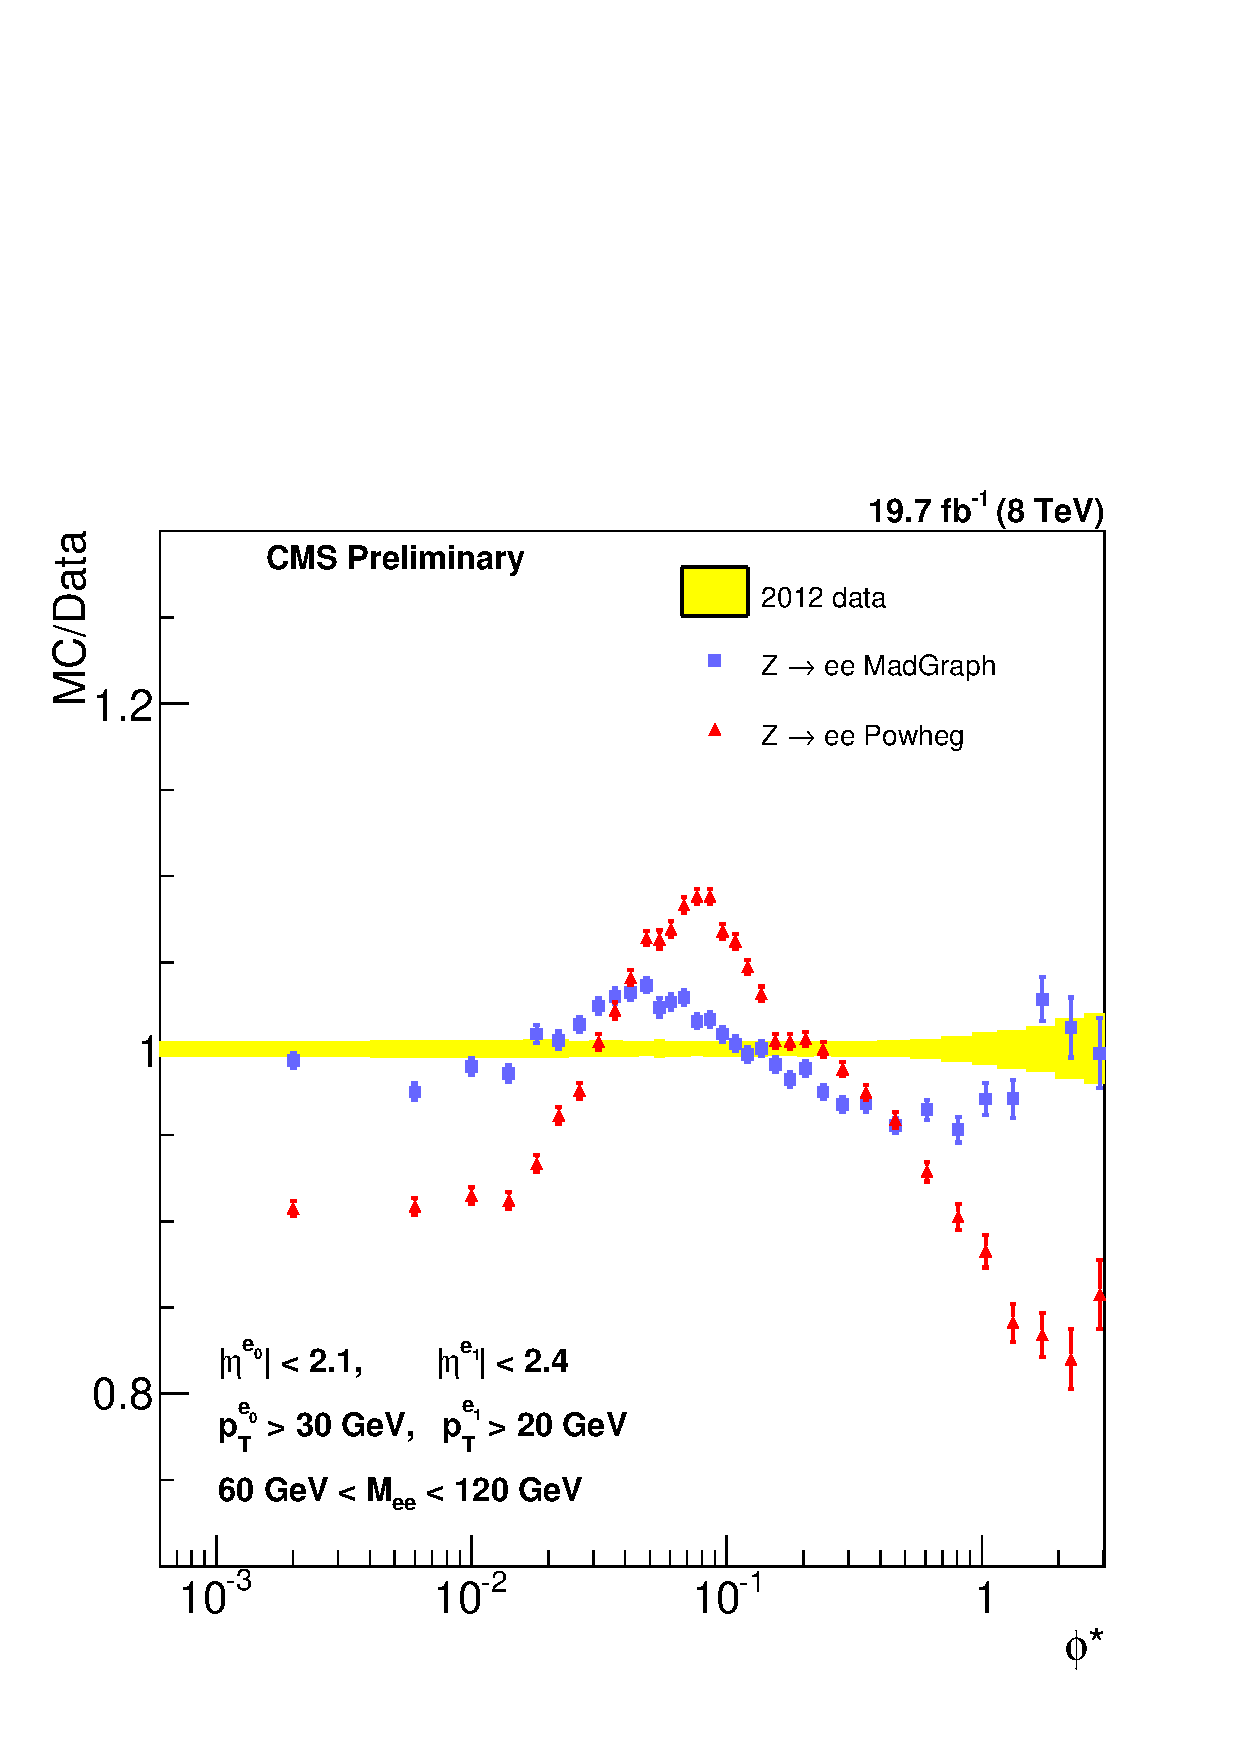
\includegraphics[width=\textwidth]{figures/ZShape_Ratioelec_Norm_Dressed.pdf}
    \caption[
        Close up of the ratio plot from \FIG~\ref{fig:results_norm} for the
        normalized cross section measurement unfolded with \MADGRAPH.
    ]{
        Close up of the ratio plot from \FIG~\ref{fig:results_norm} for the
        normalized cross section measurement unfolded with \MADGRAPH. The error
        band indicates the uncertainty in the data, while the square points
        show the ratio of \MADGRAPH over data, and the triangle points show the
        ratio of \POWHEG over data.
    }
    \label{fig:results_ratio_norm}
\end{figure}

% tab:results_norm
\begin{table}
    \spacerows{1.05}
    \begin{center}
        \begin{tabular}{@{}l r r r@{}}
            \toprule
            \phistar range & Data & \MADGRAPH & \POWHEG \\
            \midrule
            0.000--0.004  &  $9.08     \pm  0.04$     &  $9.01     \pm  0.02$     &  $8.24     \pm  0.05$     \\
            0.004--0.008  &  $9.09     \pm  0.05$     &  $8.86     \pm  0.02$     &  $8.26     \pm  0.05$     \\
            0.008--0.012  &  $8.85     \pm  0.04$     &  $8.76     \pm  0.02$     &  $8.10     \pm  0.05$     \\
            0.012--0.016  &  $8.74     \pm  0.04$     &  $8.61     \pm  0.02$     &  $7.97     \pm  0.05$     \\
            0.016--0.020  &  $8.34     \pm  0.04$     &  $8.42     \pm  0.02$     &  $7.79     \pm  0.05$     \\
            0.020--0.024  &  $8.06     \pm  0.04$     &  $8.10     \pm  0.02$     &  $7.75     \pm  0.05$     \\
            0.024--0.029  &  $7.67     \pm  0.03$     &  $7.78     \pm  0.02$     &  $7.48     \pm  0.04$     \\
            0.029--0.034  &  $7.19     \pm  0.03$     &  $7.37     \pm  0.02$     &  $7.22     \pm  0.04$     \\
            0.034--0.039  &  $6.72     \pm  0.03$     &  $6.93     \pm  0.02$     &  $6.87     \pm  0.04$     \\
            0.039--0.045  &  $6.28     \pm  0.03$     &  $6.48     \pm  0.02$     &  $6.53     \pm  0.04$     \\
            0.045--0.052  &  $5.75     \pm  0.02$     &  $5.97     \pm  0.01$     &  $6.12     \pm  0.03$     \\
            0.052--0.057  &  $5.33     \pm  0.03$     &  $5.45     \pm  0.02$     &  $5.66     \pm  0.04$     \\
            0.057--0.064  &  $4.93     \pm  0.02$     &  $5.07     \pm  0.01$     &  $5.28     \pm  0.03$     \\
            0.064--0.072  &  $4.43     \pm  0.02$     &  $4.57     \pm  0.01$     &  $4.80     \pm  0.03$     \\
            0.072--0.081  &  $4.02     \pm  0.02$     &  $4.09     \pm  0.01$     &  $4.38     \pm  0.02$     \\
            0.081--0.091  &  $3.58     \pm  0.02$     &  $3.640    \pm  0.010$    &  $3.90     \pm  0.02$     \\
            0.091--0.102  &  $3.17     \pm  0.01$     &  $3.192    \pm  0.009$    &  $3.38     \pm  0.02$     \\
            0.102--0.114  &  $2.79     \pm  0.01$     &  $2.795    \pm  0.008$    &  $2.96     \pm  0.02$     \\
            0.114--0.128  &  $2.43     \pm  0.01$     &  $2.426    \pm  0.007$    &  $2.55     \pm  0.02$     \\
            0.128--0.145  &  $2.079    \pm  0.009$    &  $2.079    \pm  0.006$    &  $2.14     \pm  0.01$     \\
            0.145--0.165  &  $1.746    \pm  0.007$    &  $1.730    \pm  0.005$    &  $1.75     \pm  0.01$     \\
            0.165--0.189  &  $1.432    \pm  0.006$    &  $1.406    \pm  0.004$    &  $1.438    \pm  0.009$    \\
            0.189--0.219  &  $1.134    \pm  0.005$    &  $1.121    \pm  0.003$    &  $1.140    \pm  0.007$    \\
            0.219--0.258  &  $0.877    \pm  0.004$    &  $0.855    \pm  0.002$    &  $0.877    \pm  0.006$    \\
            0.258--0.312  &  $0.642    \pm  0.003$    &  $0.622    \pm  0.002$    &  $0.635    \pm  0.004$    \\
            0.312--0.391  &  $0.430    \pm  0.002$    &  $0.417    \pm  0.001$    &  $0.420    \pm  0.003$    \\
            0.391--0.524  &  $0.253    \pm  0.001$    &  $0.2421   \pm  0.0007$   &  $0.243    \pm  0.002$    \\
            0.524--0.695  &  $0.1317   \pm  0.0007$   &  $0.1271   \pm  0.0004$   &  $0.1224   \pm  0.0010$   \\
            0.695--0.918  &  $0.0667   \pm  0.0005$   &  $0.0635   \pm  0.0003$   &  $0.0602   \pm  0.0006$   \\
            0.918--1.153  &  $0.0340   \pm  0.0003$   &  $0.0330   \pm  0.0002$   &  $0.0300   \pm  0.0004$   \\
            1.153--1.496  &  $0.0179   \pm  0.0002$   &  $0.0174   \pm  0.0001$   &  $0.0151   \pm  0.0003$   \\
            1.496--1.947  &  $0.0084   \pm  0.0001$   &  $0.00865  \pm  0.00007$  &  $0.0070   \pm  0.0002$   \\
            1.947--2.522  &  $0.00415  \pm  0.00007$  &  $0.00420  \pm  0.00004$  &  $0.00340  \pm  0.00009$  \\
            2.522--3.277  &  $0.00212  \pm  0.00004$  &  $0.00211  \pm  0.00003$  &  $0.00181  \pm  0.00006$  \\
            \bottomrule
        \end{tabular}
    \end{center}
    \caption[
        Normalized differential cross-section with respect to \phistar of
        \Ztoee.
    ]{
        Normalized differential cross-section with respect to \phistar of
        \Ztoee in our fiducial region in data and as generated by \MADGRAPH and
        \POWHEG. These results are shown graphically in
        figure~\ref{fig:results_norm}.
    }
    \label{tab:results_norm}
\end{table}


The normalized differential cross section measurement using data unfolded with
\POWHEG is shown in \cref{fig:results_norm_powheg} and given in tabular
form in \cref{tab:results_norm_powheg}. The lower plot in
\cref{fig:results_norm_powheg} is shown in more detail in
\cref{fig:results_ratio_norm_powheg}. The primary uncertainty on the data
is now the statistical uncertainty from the \POWHEG sample used to unfold it.

% fig:results_norm_powheg and fig:results_ratio_norm_powheg
\begin{figure}[!htbp]
    \centering
    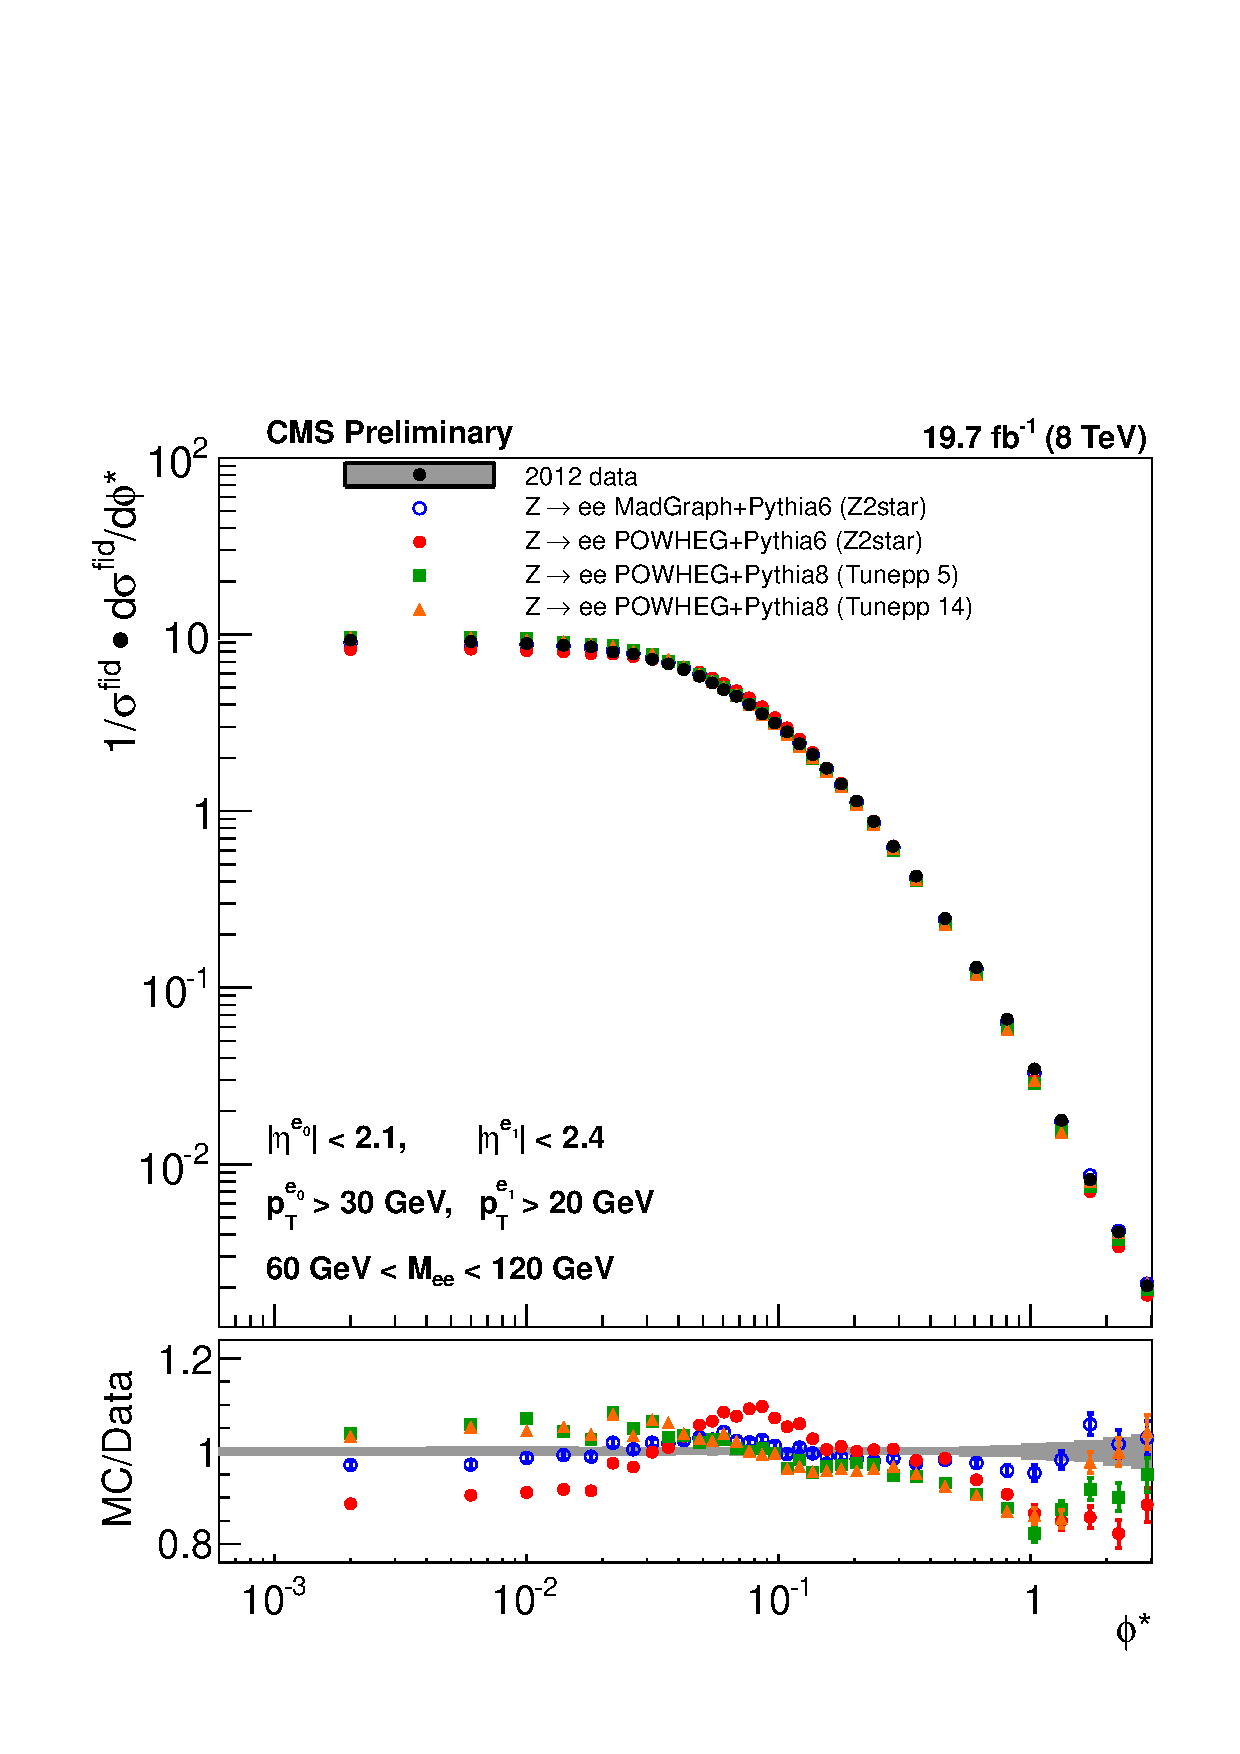
\includegraphics[width=\textwidth]{figures/ZShape_elec_PH_Norm_Dressed.pdf}
    \caption[
        The normalized differential cross section with respects to \phistar for
        \Ztoee events in our fiducial region from data and \MADGRAPH and
        \POWHEG unfolded with \POWHEG.
    ]{
        The normalized differential cross section with respects to \phistar for
        \Ztoee events in our fiducial region from data and \MADGRAPH and
        \POWHEG unfolded with \POWHEG. A close up of the lower plot is shown in
        \FIG~\ref{fig:results_ratio_norm_powheg}.
    }
    \label{fig:results_norm_powheg}
\end{figure}

\begin{figure}[!htbp]
    \centering
    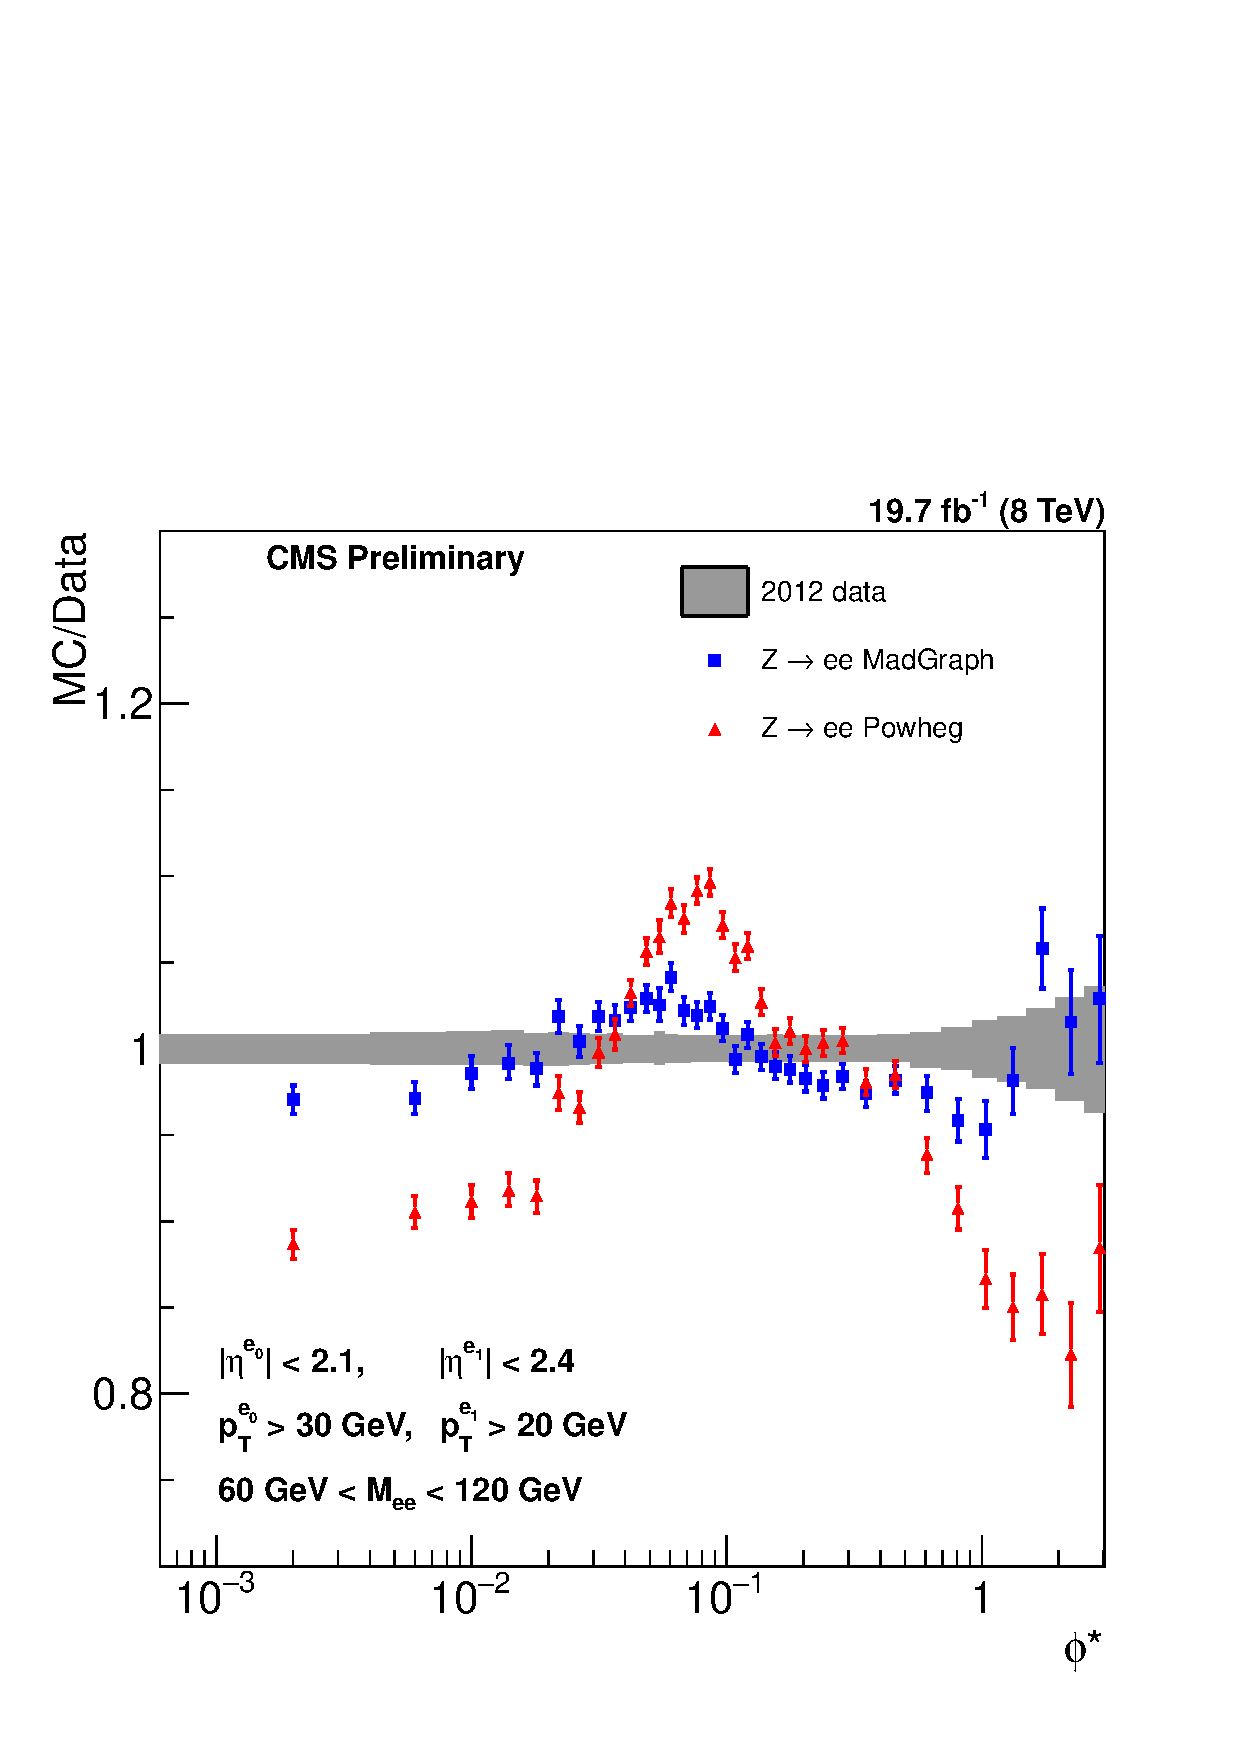
\includegraphics[width=\textwidth]{figures/ZShape_Ratioelec_PH_Norm_Dressed.pdf}
    \caption[
        Close up of the ratio plot from \FIG~\ref{fig:results_norm} for the
        normalized cross section measurement.
    ]{
        Close up of the ratio plot from \FIG~\ref{fig:results_norm} for the
        normalized cross section measurement unfolded with \POWHEG. The error
        band indicates the uncertainty in the data, while the square points
        show the ratio of \MADGRAPH over data, and the triangle points show the
        ratio of \POWHEG over data.
    }
    \label{fig:results_ratio_norm_powheg}
\end{figure}

% tab:results_norm_powheg
\begin{table}
    \spacerows{1.05}
    \begin{center}
        \begin{tabular}{@{}l r r r@{}}
            \toprule
            \phistar range & Data & \MADGRAPH & \POWHEG \\
            \midrule
            0.000--0.004  &  $9.29     \pm  0.08$     &  $9.01     \pm  0.02$     &  $8.24     \pm  0.05$     \\
            0.004--0.008  &  $9.12     \pm  0.08$     &  $8.86     \pm  0.02$     &  $8.26     \pm  0.05$     \\
            0.008--0.012  &  $8.89     \pm  0.09$     &  $8.76     \pm  0.02$     &  $8.10     \pm  0.05$     \\
            0.012--0.016  &  $8.68     \pm  0.09$     &  $8.61     \pm  0.02$     &  $7.97     \pm  0.05$     \\
            0.016--0.020  &  $8.51     \pm  0.08$     &  $8.42     \pm  0.02$     &  $7.79     \pm  0.05$     \\
            0.020--0.024  &  $7.95     \pm  0.08$     &  $8.10     \pm  0.02$     &  $7.75     \pm  0.05$     \\
            0.024--0.029  &  $7.75     \pm  0.07$     &  $7.78     \pm  0.02$     &  $7.48     \pm  0.04$     \\
            0.029--0.034  &  $7.23     \pm  0.06$     &  $7.37     \pm  0.02$     &  $7.22     \pm  0.04$     \\
            0.034--0.039  &  $6.81     \pm  0.06$     &  $6.93     \pm  0.02$     &  $6.87     \pm  0.04$     \\
            0.039--0.045  &  $6.33     \pm  0.05$     &  $6.48     \pm  0.02$     &  $6.53     \pm  0.04$     \\
            0.045--0.052  &  $5.80     \pm  0.04$     &  $5.97     \pm  0.01$     &  $6.12     \pm  0.03$     \\
            0.052--0.057  &  $5.32     \pm  0.05$     &  $5.45     \pm  0.02$     &  $5.66     \pm  0.04$     \\
            0.057--0.064  &  $4.87     \pm  0.04$     &  $5.07     \pm  0.01$     &  $5.28     \pm  0.03$     \\
            0.064--0.072  &  $4.47     \pm  0.04$     &  $4.57     \pm  0.01$     &  $4.80     \pm  0.03$     \\
            0.072--0.081  &  $4.01     \pm  0.03$     &  $4.09     \pm  0.01$     &  $4.38     \pm  0.02$     \\
            0.081--0.091  &  $3.55     \pm  0.03$     &  $3.640    \pm  0.010$    &  $3.90     \pm  0.02$     \\
            0.091--0.102  &  $3.15     \pm  0.02$     &  $3.192    \pm  0.009$    &  $3.38     \pm  0.02$     \\
            0.102--0.114  &  $2.81     \pm  0.02$     &  $2.795    \pm  0.008$    &  $2.96     \pm  0.02$     \\
            0.114--0.128  &  $2.41     \pm  0.02$     &  $2.426    \pm  0.007$    &  $2.55     \pm  0.02$     \\
            0.128--0.145  &  $2.09     \pm  0.02$     &  $2.079    \pm  0.006$    &  $2.14     \pm  0.01$     \\
            0.145--0.165  &  $1.75     \pm  0.01$     &  $1.730    \pm  0.005$    &  $1.75     \pm  0.01$     \\
            0.165--0.189  &  $1.42     \pm  0.01$     &  $1.406    \pm  0.004$    &  $1.438    \pm  0.009$    \\
            0.189--0.219  &  $1.141    \pm  0.009$    &  $1.121    \pm  0.003$    &  $1.140    \pm  0.007$    \\
            0.219--0.258  &  $0.874    \pm  0.007$    &  $0.855    \pm  0.002$    &  $0.877    \pm  0.006$    \\
            0.258--0.312  &  $0.632    \pm  0.005$    &  $0.622    \pm  0.002$    &  $0.635    \pm  0.004$    \\
            0.312--0.391  &  $0.428    \pm  0.003$    &  $0.417    \pm  0.001$    &  $0.420    \pm  0.003$    \\
            0.391--0.524  &  $0.247    \pm  0.002$    &  $0.2421   \pm  0.0007$   &  $0.243    \pm  0.002$    \\
            0.524--0.695  &  $0.130    \pm  0.001$    &  $0.1271   \pm  0.0004$   &  $0.1224   \pm  0.0010$   \\
            0.695--0.918  &  $0.0663   \pm  0.0008$   &  $0.0635   \pm  0.0003$   &  $0.0602   \pm  0.0006$   \\
            0.918--1.153  &  $0.0347   \pm  0.0006$   &  $0.0330   \pm  0.0002$   &  $0.0300   \pm  0.0004$   \\
            1.153--1.496  &  $0.0177   \pm  0.0003$   &  $0.0174   \pm  0.0001$   &  $0.0151   \pm  0.0003$   \\
            1.496--1.947  &  $0.0082   \pm  0.0002$   &  $0.00865  \pm  0.00007$  &  $0.0070   \pm  0.0002$   \\
            1.947--2.522  &  $0.0041   \pm  0.0001$   &  $0.00420  \pm  0.00004$  &  $0.00340  \pm  0.00009$  \\
            2.522--3.277  &  $0.00205  \pm  0.00007$  &  $0.00211  \pm  0.00003$  &  $0.00181  \pm  0.00006$  \\
            \bottomrule
        \end{tabular}
    \end{center}
    \caption[
        The normalized differential cross section in \pb with respects to
        \phistar for \Ztoee events in our fiducial region from data unfolded
        with \POWHEG.
    ]{
        The normalized differential cross section in \pb with respects to
        \phistar for \Ztoee events in our fiducial region from data unfolded
        with \POWHEG, and the same distributions in \MADGRAPH and \POWHEG.
        These results are shown graphically in \cref{fig:results_norm_powheg}.
    }
    \label{tab:results_norm_powheg}
\end{table}


\clearpage
\section{Discussion and Conclusion}
\label{sec:discussion}

A measurement of the normalized differential cross section of the \Z boson
decaying to electron pairs in terms of \phistar was performed using
\GoodLumiNumber of \rootseight data collected with the CMS detector. This
measurement was compared to the predictions from the \MADGRAPH and \POWHEG
generators.

The prediction from \MADGRAPH is everywhere within 5\% of the distribution
measured in data unfolded with \MADGRAPH. The generator underestimates the
cross section in both the low and high \phistar bins, but agrees in the very
lowest bin and the three highest bins. In the intermediate region, \MADGRAPH
switches from underestimating to overestimating the cross section, but does so
smoothly. Surprisingly, the prediction from \MADGRAPH agrees better with the
data unfolded with \POWHEG, and not just because the uncertainty is larger. The
central value of the prediction from \MADGRAPH is closer to the data even
disregarding the uncertainty.

The prediction from \POWHEG is significantly worse than the prediction from
\MADGRAPH. Compared to the \MADGRAPH unfolded data, \POWHEG's prediction
underestimate the cross section by 10\% in the low \phistar region, 15\% in the
high \phistar region, and overestimates the cross section by 10\% in the
intermediate region. In fact \POWHEG is only consistent with the data in five
bins, although four of these are grouped together around $\phistar \approx
0.15$. \POWHEG does equally poorly when compared with the data unfolded with
\POWHEG.

The \phistar variable, as expected, had very limited dependence on the \pt
scale uncertainty of the detector, which was the smallest of the systematic
uncertainties considered. Still, the measurement was limited by the systematic
uncertainties, particularly the small number of MC events used for the
unfolding. Fortunately, reducing this uncertainty is easy (although
computationally expensive) as all that is required is to generate additional MC
events. The statistical uncertainties were the next largest uncertainty. As the
remaining uncertainties were all vanishingly small, future versions of this
analysis will be able to improve on the measurement without needing to develop
new analysis techniques.
